\documentclass[ngerman]{gdb-aufgabenblatt}
\usepackage{enumitem}
\usepackage{dingbat}
\usepackage{ifsym}
\usepackage{amssymb}
\usepackage{amsmath}
\renewcommand{\Aufgabenblatt}{4}
\renewcommand{\Ausgabedatum}{Mi. 15.11.2017}
\renewcommand{\Abgabedatum}{Fr. 12.1.2018}
\renewcommand{\Gruppe}{Meimerstorf,Jochens,T�ter}
\renewcommand{\STiNEGruppe}{19}
\usepackage{tabularx}
\usepackage[normalem]{ulem}

\begin{document}

\section{Referentielle Aktion}
\subsection{}
\begin{center}
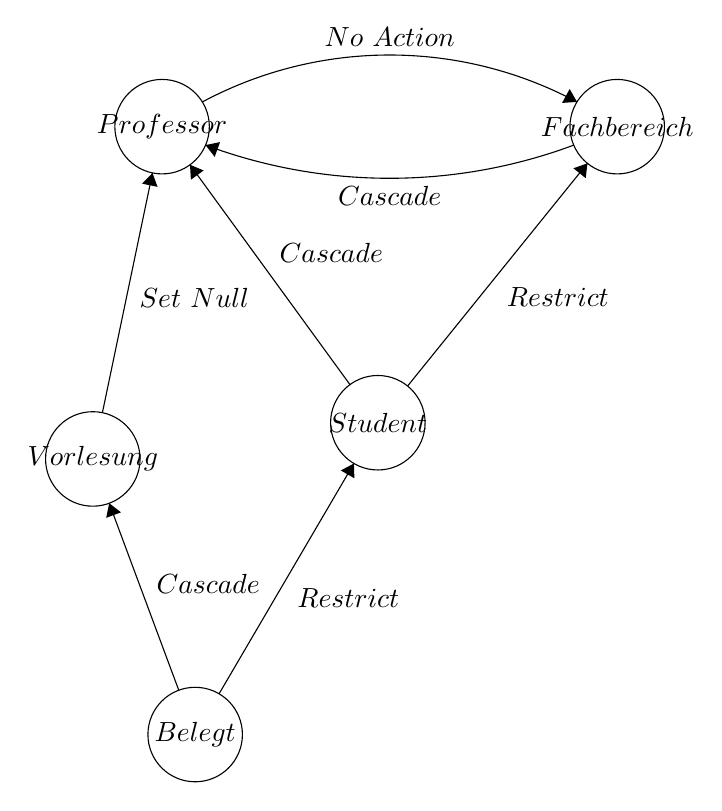
\begin{tikzpicture}[scale=0.2]
\tikzstyle{every node}+=[inner sep=0pt]
\draw [black] (10.1,-8.4) circle (3);
\draw (10.1,-8.4) node {$Professor$};
\draw [black] (23.8,-27.2) circle (3);
\draw (23.8,-27.2) node {$Student$};
\draw [black] (39,-8.4) circle (3);
\draw (39,-8.4) node {$Fachbereich$};
\draw [black] (5.7,-29.5) circle (3);
\draw (5.7,-29.5) node {$Vorlesung$};
\draw [black] (12.2,-47) circle (3);
\draw (12.2,-47) node {$Belegt$};
\draw [black] (22.03,-24.78) -- (11.87,-10.82);
\fill [black] (11.87,-10.82) -- (11.93,-11.77) -- (12.74,-11.18);
\draw (17.53,-16.42) node [right] {$Cascade$};
\draw [black] (12.655,-6.831) arc (118.14753:61.85247:25.215);
\fill [black] (36.45,-6.83) -- (35.98,-6.01) -- (35.5,-6.89);
\draw (24.55,-3.35) node [above] {$No\mbox{ }Action$};
\draw [black] (13.72,-44.41) -- (22.28,-29.79);
\fill [black] (22.28,-29.79) -- (21.45,-30.23) -- (22.31,-30.73);
\draw (18.65,-38.34) node [right] {$Restrict$};
\draw [black] (11.16,-44.19) -- (6.74,-32.31);
\fill [black] (6.74,-32.31) -- (6.55,-33.24) -- (7.49,-32.89);
\draw (9.71,-37.44) node [right] {$Cascade$};
\draw [black] (6.31,-26.56) -- (9.49,-11.34);
\fill [black] (9.49,-11.34) -- (8.83,-12.02) -- (9.81,-12.22);
\draw (8.64,-19.29) node [right] {$Set\mbox{ }Null$};
\draw [black] (36.239,-9.572) arc (-69.56917:-110.43083:33.487);
\fill [black] (12.86,-9.57) -- (13.44,-10.32) -- (13.78,-9.38);
\draw (24.55,-12.18) node [below] {$Cascade$};
\draw [black] (25.69,-24.87) -- (37.11,-10.73);
\fill [black] (37.11,-10.73) -- (36.22,-11.04) -- (37,-11.67);
\draw (31.96,-19.23) node [right] {$Restrict$};
\end{tikzpicture}
\end{center}
\subsection{}
Falls man einen Professor l�scht, und dann als erstes, der Student gel�scht wird, l�uft man je nach Reihenfolge entweder in das Restrict beim Belegt oder wenn man als erstes den Fachbereich l�scht, in das Restrict beim Studenten, bzw. wenn der Student vorher schon gel�scht wurde, w�rde hierbei nicht einmal das Restrict. \\
Abschlie�end also kein sicheres Schema. \\
\subsection{}
\begin{verbatim}
ALTER TABLE `Student` 
DROP FOREIGN KEY `fkFachbereich`;  
\end{verbatim}
\begin{verbatim}
ALTER TABLE `table1` 
ADD CONSTRAINT `fkFachbereich` FOREIGN KEY (`Fachbereich`) REFERENCES
 `Fachbereich` ON DELETE CASCADE;   
\end{verbatim}
\subsection{}
Ja
\section{�nderbarkeit von Sichten}
\subsection{}
\begin{verbatim}
Create View GesamtwerkB�ll
	AS SELECT b.ISBN,b.TITEL 
	FROM Buch b , Schriftsteller autor  
		WHERE b.Autor = Autor.Snr 
		AND autor.Nachname = 'B�ll'
		AND autor.Vorname  = 'Heinrich'
\end{verbatim}
Operationen nicht zul�ssig, zwei Tabellen.

\begin{verbatim}
Create View AlteBritischeAutoren
	AS SELECT Snr,Vorname,Nachname 
	FROM Schriftsteller   
		WHERE Nationalit�t = 'britisch' 
		AND Geburtsjahr < 1960 
\end{verbatim}
Operationen zul�ssig SNR ist dabei.


\begin{verbatim}
Create View B�cherHeyne
	AS SELECT Titel 
	FROM Buch   
		WHERE VERLAG = "Heyne'
\end{verbatim}
Nicht zul�ssig, schl�ssel fehlt. 
\subsection{}
\begin{itemize}
\item i)
zul�ssig\\
Nur in SciFiKlassiker Fischer k�nnen neue auftreten.
\item ii)
zul�ssig
In SciFiKlassiker Fischer und in SciFiKlassiker k�nnen neue auftreten.\\
\item iii)\\
Fehler durch Cascaded Vererbte Check Option bei Klassiker.
\item iv)\\
Kein Fehler, da einf�gen direkt in Klassiker den Check nicht ausl�st. \\
Werden in allen sichtbar. 
\end{itemize}
\section{Serialisierbarkeit, Anomalien}
\subsection{}
\begin{itemize}
\item $S_1$ Endwert: A:30 B:130
\item $S_2$ Endwert: A:10 B:120
\item $S_3$ Endwert: A:10 B:200
\item $S_4$ Endwert: A:10 B:120	
\item $S_5$ Endwert: A:10 B:20
\item $S_6$ Endwert: A:10 B:110
\end{itemize}
\subsection{}
Abh�ngikeiten hier allgemein gehalten, welche entsehen k�nnen und nicht f�r jede einzelne Schedule. Da zu faul. (Genaue Abh�ngikeiten bei c).\\
Bei den Transaktionen besteht die Abh�ngikeit dabei, dass sie beide auf den Werten a/b agieren. Das hei�t wenn die eine Transaktion einen Wert eingelesen hat, bevor die andere Transaktion ihren aktuellen Wert zur�ckgeschrieben hat, kommt es zu einer Anomalie, da die erste Transaktionen einen dreckigen Wert liest und mit dem weiterrechnet. \\
Also muss die w-Operation einer Transaktion immer vor der n�chsten Lese Operation auf den Wert ausgef�hrt werden. \\	
\subsection{}
\begin{itemize}
\item $S_1$ Seriell (hintereinander weggearbeitet)
\item $S_2$ Seriell (hintereinander weggearbeitet)
\item $S_3$ nicht serialisierbar(r1 lie�t bevor r2 schreibt bzw. r2 liest bevor w1 schreibt)
\item $S_4$ serialisierbar (die reads der anderen Transaktion treten immer erst auf nachdem die andere geschrieben hat)
\item $S_5$ nicht serialisierbar(r1 lie�t bevor r2 schreibt bzw. r2 liest bevor w1 schreibt)
\item $S_6$ nicht serialisierbar(r1 lie�t bevor r2 schreibt bzw. r2 liest bevor w1 schreibt und au�erdem liest r1 auch A bevor w2 schreibt.)
\end{itemize}
\section{2PL-Synchronisation mit R/X-Sperre}
\begin{center}
 \begin{tabular}{|c|c|c|c|c|}
    \hline 
     & $T_1$ & $T_2$ & $T_3$ & Bemerkung \\ 
    \hline 
    0 &  &  &  &  \\ 
    \hline 
    1 &  &  & lock(x,X) &  \\ 
    \hline 
    2 &  &  & write(x) &  \\ 
    \hline 
    3 &  &  & lock(y,R) & \\ 
    \hline 
    4 & lock(x,R) &  & read(y) &  \\ 
    \hline 
    5 & read(x) & lock(y,R) &  &  \\ 
    \hline 
    6 &  & read(y) & lock(y,X) & T3 wartet T2 \\ 
    \hline 
    7 & lock(x,X) &  &  & \\ 
    \hline 
    8 & write(x) & lock(z,R) &  &  \\ 
    \hline 
    9 & unlock(x) & read(z) &  &  \\ 
    \hline 
    10 & commit & unlock(y) &  & Nachricht an T3 \\ 
    \hline 
    11 &  & unlock(z) & write(y) &  \\ 
    \hline 
    12 &  & commit & lock(x,R) &  \\ 
    \hline 
    13 &  &  & read(x) &  \\ 
    \hline 
    14 &  &  & unlock(y) &  \\ 
    \hline 
    15 &  &  & unlock(x) &  \\ 
    \hline 
    16 &  &  & commit &  \\ 
    \hline 
    17 &  & &  &  \\ 
    \hline 
    \end{tabular} 
\end{center}
\end{document}